\documentclass[a4paper,11pt]{article}
\usepackage[margin=1.5cm]{geometry}
\usepackage{amsmath}
\usepackage{amssymb}
\usepackage{color}
\usepackage{graphicx}
\usepackage{graphics}
\usepackage[margin=1.5cm]{geometry}
\usepackage{fancyhdr}
\usepackage{float}
\usepackage{wrapfig}
\usepackage{lscape}
\usepackage[font={small},labelfont=bf]{caption}
\usepackage{palatino}
\usepackage{mathpazo}

\bibliographystyle{unsrt}
%\linespread{1.2}

%%%%%%%
%Defines vectors universally, for ease of editing and consistency.
\newcommand{\vtr}[1] {\mathit{\underline{\boldsymbol{#1}}}}

%Draws a big red box containing the text as in \ALERT{<TEXT HERE>}. For labelling draft copies with important notes.
\def\ALERT#1{\begin{center}\colorbox{red}{\hbox{\textcolor{black}{\textbf{#1}}}}\end{center}}

%Roman-style subscript; removes math-mode font.
\def\s#1{_\textrm{#1} }

%The operators in integrals and derivatives.
\def\d{\operatorname{d}\!}

%The Euler e should be in Roman font.
\def\e{\textrm{e}}

%%%%%%%%%%%   some definitions used in latexing the CQMP:
% fractions that are of right size in set equations
\def\half{{\textstyle \frac{1}{2}}}
\def\quarter{{\textstyle \frac{1}{4}}}
\def\third{{\textstyle \frac{1}{3}}}
\def\eighth{{\textstyle \frac{1}{8}}}

% obtain a new line
\def\nl{\hfil\break}
\def\nll{\\ \\ \noindent}
%%%%%%%%%

%******************************* to optimise page usage
%\setlength{\textwidth}{6.3 in}

%\setlength{\oddsidemargin}{0.2 in}
%\setlength{\evensidemargin}{0.2 in}

%\setlength{\topmargin}{-.80 in}
%\setlength{\textheight}{9.9 in}
%*******************************
% to mark as a draft.  Comment both these lines out when complete.  The page number will return to the footer.
%\pagestyle{myheadings}
\markright{\textcolor{red}{\textbf{DRAFT: \today}}}




\begin{document}
\setlength{\columnsep}{22pt}
%\vspace{-5cm}
%\maketitle
\textsc{\center \Large  Physical Concept: \textbf{Momentum and its conservation; collisions.}}
\vspace{0.7cm}

We briefly sketch definitions of momentum.  Understanding momentum further involves revising Newton's Laws and ideas about impulse, which are available at greater length at the concepts pages for Newton's Laws and for Impulse.  Collisions are a good area for illustration.

\section{Definition of momentum}

Momentum is mass $m$ times velocity $\vtr{v}$ for a particle: $\boxed{\vtr{p} = m \vtr{v}}$.\\
%\begin{equation*} \boxed{\vtr{p} = m \vtr{v}}
%\end{equation*}
It is a vector with units kg.m/sec.  Momentum can be carried by other entities, such as waves, but we just sketch mechanical momentum.

\section{Conservation of momentum}

The momentum is conserved in the absence of forces external to the system.  \\
This concept is one of the most important in physics and follows from Newton's laws.  Newton's second law (N2L, ``force = mass times acceleration") can be written:
\begin{equation*} \vtr{f} = m \vtr{a} = m \d\vtr{v}/\d t = \d\vtr{p}/\d t .
\end{equation*}
N1L says that in the absence of forces, particles continue moving without further change of velocity.  Setting $\vtr{f}= 0$ in the above shows that then $\vtr{v}$ is unchanging, as is momentum $\vtr{p}$, that is momentum is conserved.\\
\begin{wrapfigure}{r}{6cm}\vspace{-1cm}
\center
\includegraphics[width=0.3\textwidth]{collision.eps}
\caption{The collision of two particles isolated from the rest of the world.}
\label{fig:collision}
\end{wrapfigure}
Consider a system consisting of two particles colliding head on, figure~\ref{fig:collision}. The box indicates the system is ``closed" --- there are forces within it (when the particles collide), but not on it from outside.

Momentum is always conserved, but energy can be converted to other forms (e.g. to heat) so collisions may or may not be elastic (that is conserving mechanical energy).  So one has:
\begin{equation*} \vtr{p}_1 +  \vtr{p}_2 = \vtr{p}_1'  + \vtr{p}_2'
\end{equation*}
where the prime $'$ indicates after the collision.

\nl
{\bf Levels 1--4.  Examples}
\nl
1.  Figure~\ref{fig:inelastic} shows two particles colliding and then sticking together.

 \begin{wrapfigure}{r}{5cm}
\center
\includegraphics[width=0.25\textwidth]{inelastic.eps}
\caption{The inelastic collision of two particles that stick together after colliding.}
\label{fig:inelastic}
\end{wrapfigure}
If $m_1 = 1 \textrm{kg}$, $m_2 = 2\textrm{kg}$, $v_1 = 3 \textrm{m s}^{-1}$ and
$v_2 = 1\textrm{m s}^{-1}$, then the momentum is $1 \times 3 + 2 \times 1  = 5 \textrm{kg m s}^{-1}$.
It remains this value and hence after the collision one has $5 \textrm{kg m s}^{-1} = 3 \textrm{kg} \times v' \; \textrm{m s}^{-1}$.  Thus $ v' = 5/3 \; \textrm{m s}^{-1}$.
\nl
Calculate how much energy has been lost in the collision by calculating the total kinetic energy before and after.\\
Describe the collision (with sticking) in the case $m_1 = m_2 = 1\textrm{kg}$.
\begin{wrapfigure}{r}{5cm} 
\center
\includegraphics[width=0.25\textwidth]{elastic.eps}
\caption{An elastic collision of two equal particles, one being initially at rest.}
\label{fig:elastic}
\includegraphics[width=0.2\textwidth]{wall.eps}
\caption{A particle colliding with a wall.  In the intermediate state it is instantaneously at rest and deformed.} \vspace{-1.0cm}
\label{fig:wall}
\end{wrapfigure}

\nl
2.  Consider two particles of equal mass, $m_1 = m_2 = m$ where $v_1 = v$ simply, and the other particle is initially at rest, $v_2=0$.  They collide elastically; see figure~\ref{fig:elastic}.  What are the final speeds $v_1'$ and $v_2'$?

\nl Conserving momentum gives: $m v = m (v_1' + v_2')$ hence $v = v_1' + v_2'$.\\
Conserving energy gives: $\half m v^2 = \half m (v_1'^2 + v_2'^2)$.  Hence
$v^2 = v_1'^2 + v_2'^2$.
\nl
Put $v_1'  = v - v_2'$ from above into this energy relation:
\begin{equation*} v^2 = (v - v_2')^2 + v_2'^2  = v^2 - 2 v v_1' +v_1'^2 + v_1'^2\\
\rightarrow 2 v v_2' = 2 v_2'^2  \rightarrow v_2' = v .
\end{equation*}
Put this value of $v_2'$ into the momentum relation and find that $v_1' = 0$.
\nl
The first particle stops and the second continues with the velocity (and momentum) of the first --- like in Newton's cradle.

\nl
3.  A particle bouncing off a wall; figure~\ref{fig:wall}.\\

The incident particle has a force from the wall acting on it during the collision.  Momentum of the particle is not conserved. But \textit{the total momentum} of the particle plus the wall \textit{is conserved}.\\
  What is the change of momentum if the collision is elastic? (Remember momentum and its changes are vectors -- your answer requires a magnitude and a direction.)\\
 What is the momentum change if the collision is completely inelastic?


\section{Impulse}
Impulse is the change of momentum.  It is force times time, for a constant force acting.  The term is generally (but not always) used when momentum is transferred over a short time (e.g. during a collision).  It is described fully in the impulse concepts sheet.
\section{Level 5+: Zero Momentum Frame}
\begin{wrapfigure}{r}{9cm}
\vspace{-1.0cm}
\includegraphics[width=0.5\textwidth]{ZMF1.eps}
\caption{A table of diagrams showing how we use the zero momentum frame (ZMF) to calculate the result of a {\it perfectly inelastic}, head-on, collision between two equal masses where one is at rest and the other travelling at velocity, $v$.  To move from (a) to (b) we subtract the velocity of the zero momentum frame.  To move from (b) to (c) in the zero momentum frame the only way to conserve momentum in a head-on, perfectly inelastic collision, is if the magnitude of the velocity of the combined mass, $2m$, is zero.  To return to the lab frame, (c) to (d), we must then add back on the velocity of the zero momentum frame to this combined mass.}
\label{fig:ZMF1}
\end{wrapfigure}
The zero momentum frame is a construct that physicists use to simplify the algebra that is involved in collision calculations where momentum is conserved.  By transferring to a frame in which the total momentum of the system is zero we can remove the need to solve simultaneous equations for energy and momentum.\\

\noindent{\bf Example 4:}  A perfectly inelastic head on collision between equal masses, one at rest the other at velocity $v$. (Also explained in figure \ref{fig:ZMF1})\\

\noindent We will begin by taking the simplest example where a mass, $m$, travelling at velocity, $v$, collides head-on, and {\it perfectly inelastically}, with an object of the same mass, $m$, which is at rest (previous example 1, as shown in figure \ref{fig:inelastic}).\\

\noindent Because the zero momentum frame removes the need for any detailed algebra in simple cases, figure \ref{fig:ZMF1} essentially performs the calculation for us.  We will refer therefore to two frames which we can imagine as the platform at a train station and a train passing through the station.
The first, the station platform, is the laboratory (lab) frame where the collision is happening.  The second, the train passing through the station at a specific velocity in the same direction as the moving mass, is zero momentum frame.  An observer on the {\it platform} sees one mass moving at $v$ and one at rest,  imagine that you are on that train how will the velocities of masses appear to you? \\

\noindent First of all we need to calculate the specific velocity of the zero momentum frame (the train) such that the total momentum in this frame is zero.  To do this we need to calculate the total momentum of the system and divide by the total mass.

\addtocounter{figure}{-1}
\begin{wrapfigure}{r}{9cm}
\includegraphics[width=0.5\textwidth]{ZMF1.eps}
\caption{A table of diagrams showing how we use the zero momentum frame (ZMF) to calculate the result of a {\it perfectly inelastic}, head-on, collision between two equal masses where one is at rest and the other travelling at velocity, $v$.  To move from (a) to (b) we subtract the velocity of the zero momentum frame.  To move from (b) to (c) in the zero momentum frame the only way to conserve both energy and momentum in a head-on, inelastic collision, is if the magnitude of the velocity of the combined mass, $2m$, is zero.  To return to the lab frame, (c) to (d), we must then add back on the velocity of the zero momentum frame to this combined mass.}\vspace{1cm}
\label{fig:ZMF1}
\includegraphics[width=0.5\textwidth]{ZMF2.eps}
\caption{A table of diagrams showing how we use the zero momentum frame (ZMF) to calculate the result of an {\it elastic}, head-on, collision between two equal masses where one is at rest and the other travelling at velocity, $v$.  To move from (a) to (b) we subtract the velocity of the zero momentum frame.  To move from (b) to (c) in the zero momentum frame the only way to conserve both energy and momentum in a head-on, elastic collision, is if the magnitude of the velocities remains the same but the direction is reversed.  To return to the lab frame, (c) to (d), we must then add back on the velocity of the zero momentum frame.} 
\label{fig:ZMF2} 
\end{wrapfigure}

\begin{equation}
v_{zmf}=\frac{\sum_i{m_i v_i}}{\sum_i m_i} = \frac{mv+0}{2m} = \frac{v}{2}
\end{equation}

\noindent To work out what the observer on the train (in the ZMF) sees we need to subtract the speed of the train from each mass so in figure \ref{fig:ZMF1} we move from (a) to (b) by subtracting $v/2$ to the right.  Therefore mass 1 in the ZMF has velocity
\begin{equation}
v-v_{zmf}=v-\frac{v}{2}=\frac{v}{2}
\end{equation}
Mass 2 in the ZMF has velocity
\begin{equation}
0-v_{zmf}=-\frac{v}{2}\ \  \mbox{which is the same as}\ \frac{v}{2}\ \mbox{to the left}.
\end{equation}
\\
\noindent In a perfectly inelastic collision the two individual masses must stick together to make one object of mass $2m$.  If we have just one object in the zero momentum frame there is only one was that the momentum can be conserved as zero - if the velocity of this $2m = 0$! \\

\noindent To return to the lab frame we must then add back on the velocity of the ZMF. So, defining velocities to the right as positive, the velocity of the $2m$ is now
\begin{equation}
0+v_{zmf}=\frac{v}{2} \ \mbox{to the right}
\end{equation}
as shown in figure \ref{fig:ZMF1} (d).  After such a calculation you should always check that momentum is conserved between the lab frame before and after the collision. 
\\
\\
{\bf Example 5:} An elastic head on collision between equal masses, one at rest the other at velocity $v$. (Also explained in figure \ref{fig:ZMF2}).
\\
\\
In this example we have a a mass, $m$, travelling at velocity, $v$, collides head-on, and {\it elastically}, with an object of the same mass, $m$, which is at rest (previous example 2, as shown in figure \ref{fig:elastic}).
\nll
By the same reasoning as that in example 4, the velocities of the two masses in the zero momentum frame are equal in magnitude, $v/2$, but opposite in direction.  In the {\it inelastic} example the zero momentum frame was useful as we could quickly reason that after the collision the velocity of the combined mass, $2m$ must be zero in the ZMF.  The reason that we use the ZMF for an {\it elastic} head-on collision is that the the only way to conserve both momentum ($=0$) and energy in this frame is if the magnitude of the velocities remain the same but the direction of each {\it after} the collision is reversed.  Therefore {\it no} further calculation is required.
\nll
To return to the laboratory frame we just add back on the velocity of the zero momentum frame (as before), which in our example is $v/2$ to the right. 
\begin{wrapfigure}{rt}{9.0cm}
\vspace{-21.5cm}
\includegraphics[width=0.5\textwidth]{ZMF1a.eps}
\caption{A table of diagrams showing how we use the zero momentum frame (ZMF) to calculate the result of a {\it perfectly inelastic}, head-on, collision between two masses, $m$ and $2m$, where $m$ is travelling at velocity $v$ and mass $2m$ is at rest.  To move from (a) to (b) we subtract the velocity of the zero momentum frame.  To move from (b) to (c) in the zero momentum frame the only way to conserve both energy and momentum in a head-on, inelastic collision, is if the magnitude of the velocity of the combined mass, $2m$, is zero.  To return to the lab frame, (c) to (d), we must then add back on the velocity of the zero momentum frame to this combined mass.}\vspace{1cm}
\label{fig:ZMF1a}
\includegraphics[width=0.5\textwidth]{ZMF2a.eps}
\caption{A table of diagrams showing how we use the zero momentum frame (ZMF) to calculate the result of a {\it perfectly inelastic}, head-on, collision between two masses, $m$ and $2m$, where $m$ is travelling at velocity $v$ and mass $2m$ is at rest.  To move from (a) to (b) we subtract the velocity of the zero momentum frame.  To move from (b) to (c) in the zero momentum frame the only way to conserve both energy and momentum in a head-on, inelastic collision, is if the magnitude of the velocity of the combined mass, $2m$, is zero.  To return to the lab frame, (c) to (d), we must then add back on the velocity of the zero momentum frame to this combined mass.}
\label{fig:ZMF2a}
\end{wrapfigure}
 \\
We define the positive direction as to the right so, for mass 1
\begin{equation}
-\frac{v}{2}+v_{zmf}=-\frac{v}{2}+\frac{v}{2}=0
\end{equation}
and mass 2 in the lab frame has velocity
\begin{equation}
\frac{v}{2}+v_{zmf}=\frac{v}{2}+\frac{v}{2} =v\ \  \mbox{to the right}.
\end{equation}
\\
\noindent{\bf Example 6:} A perfectly inelastic collision between a mass, $m$, travelling at velocity, $v$, and a mass, $2m$, that is stationary. (Also explained in figure \ref{fig:ZMF1a})\nll
As before the only real calculation that is required is to compute the velocity of the zero momentum frame.
\begin{equation}
v_{zmf}=\frac{mv}{3m}=\frac{v}{3}
\end{equation}
We can now follow the process once again, through figure \ref{fig:ZMF1a}, subtracting the velocity of the ZMF from the velocity of each mass to become an observer in the ZMF.  For a perfectly inelastic collision the masses must join together and become one so we know that the velocity of these combined masses must be zero in the ZMF.  The final step therefore is to add back on the velocity of the ZMF to return to the laboratory frame.  Thus the combined $3m$ mass must be travelling with velocity $v/3$ and we check again that momentum is conserved in the lab frame before and after the collision.\\

\noindent{\bf Example 7:} A perfectly elastic collision between a mass, $m$, travelling at velocity, $v$, and a mass, $2m$, that is stationary. (Also explained in figure \ref{fig:ZMF2a}\\

\noindent The left hand side of our diagram, before the collision, is the same as for the inelastic case.    For a perfectly elastic collision we know that the magnitude of the velocities remain the same but the directions are reversed.  The final step therefore is to add back on the velocity of the ZMF to return to the laboratory frame.  Thus the particle of mass $m$ must bounce back to the left with velocity $v/3$ and the particle of mass $2m$ moves off with velocity $2v/3$ to the right.
\pagebreak
\section{Level 6}
\begin{wrapfigure}{rt}{9.0cm}
\includegraphics[width=0.5\textwidth]{ZMF3.eps}
\caption{A table of diagrams showing how we use the zero momentum frame (ZMF) to calculate the result of a {\it perfectly inelastic}, head-on, collision between two general masses $m_1$ and $m_2$ travelling at velocities, $v_1$ and $v_2$ respectively.  To move from (a) to (b) we subtract the velocity of the zero momentum frame.  To move from (b) to (c) in the zero momentum frame the only way to conserve momentum in a, perfectly inelastic collision, is if the velocity of the combined particle is zero.  To return to the lab frame, (c) to (d), we must then add back on the velocity of the zero momentum frame.}\vspace{1cm}
\label{fig:ZMF3}
\includegraphics[width=0.5\textwidth]{ZMF4.eps}
\caption{A table of diagrams showing how we use the zero momentum frame (ZMF) to calculate the result of a {\it perfectly elastic}, head-on, collision between two general masses $m_1$ and $m_2$ travelling at velocities, $v_1$ and $v_2$ respectively.  To move from (a) to (b) we subtract the velocity of the zero momentum frame.  To move from (b) to (c) in the zero momentum frame the only way to conserve momentum in a, perfectly elastic collision, is if the magnitude of the velocities of each particle remain the same but the directions are reversed.  To return to the lab frame, (c) to (d), we must then add back on the velocity of the zero momentum frame.}
\label{fig:ZMF4}
\end{wrapfigure}
By generalisation we can use the zero momentum frame for two particles of different masses and different, non-zero velocities, in both elastic and inelastic cases.
\nll
{\bf Example 8:} A perfectly inelastic collision of masses, $m_1$ and $m_2$ with respective velocities $v_1$ and $v_2$.  (Also explained in figure \ref{fig:ZMF3}).
\nll
The process for the general case is identical to that of the specific cases and most of the work will be done using the table of diagrams as before.  The first thing is to calculate the velocity, $v_{zmf}$ of the zero momentum frame.
\begin{equation}
v_{zmf}=\frac{m_1 v_1+m_2 v_2}{m_1 +m_2}
\end{equation}
\noindent
We know that the velocity of the combined mass after the perfectly inelastic collision must be zero in the zero momentum frame so the velocity of the combined mass in the lab frame is therefore just the velocity of the zero momentum frame.
\begin{equation}
\mbox{final lab frame velocity}=\frac{m_1 v_1+m_2 v_2}{m_1 +m_2}
\end{equation}
\noindent
{\bf Example 9:} Perfectly elastic collision of masses, $m_1$ and $m_2$ with respective velocities $v_1$ and $v_2$.   (Also explained in figure \ref{fig:ZMF4}).
\\
\\
Once again we calculate the velocity, $v_{zmf}$ of the zero momentum frame, which as in the inelastic case is,
\begin{equation}
v_{zmf}=\frac{m_1 v_1+m_2 v_2}{m_1 +m_2}
\end{equation}
\noindent
We know that the magnitudes of the velocities of each particle must remain the same after the collision but that their directions must reverse.  To return to the lab frame we must add back on the velocity of the zero momentum frame so that in the lab frame the
\begin{eqnarray}
\mbox{final velocity of $m_1$}=\frac{v_1(m_1-m_2)+2m_2v_2}{m_1 +m_2}\nonumber\\
\mbox{final velocity of $m_2$}=\frac{v_2(m_2-m_1)+2m_1v_1}{m_1 +m_2}\nonumber\\
\end{eqnarray}
You should now convince yourself that these statements are correct for examples 6 and 7 in the previous level 5+ section.

\end{document}
